\documentclass[a4paper]{scrartcl}
\usepackage{fancyhdr}
\pagestyle{fancy}
\usepackage[english]{babel}
\usepackage[utf8]{inputenc}
\usepackage{graphicx}
\usepackage{url}
\usepackage{textcomp}
\usepackage{amsmath}
\usepackage{lastpage}
\usepackage{pgf}
\usepackage{wrapfig}
\usepackage{fancyvrb}

% Listing header

\usepackage{listings}
\usepackage{xcolor}

\definecolor{lightgray}{gray}{0.95}

\lstdefinestyle{javastyle}{
    backgroundcolor=\color{lightgray},
    basicstyle=\ttfamily\small,
    numbers=left,
    numberstyle=\tiny,
    numbersep=8pt,
    frame=single,
    showstringspaces=false,
    breaklines=true,
    breakautoindent=true,
    breakindent=2em,
    keepspaces=true,
    columns=fullflexible,
    tabsize=4,
    language=Java,
    keywordstyle=\color{blue},
    commentstyle=\color{gray!70},
    stringstyle=\color{orange!90!black}
}

% Create header and footer
\headheight 27pt
\pagestyle{fancyplain}
\lhead{\footnotesize{Object-Oriented Design, IV1350}}
\chead{\footnotesize{Seminar 2 Solution}}
\rhead{}
\lfoot{}
\cfoot{\thepage\ (\pageref{LastPage})}
\rfoot{}

% Create title page
\title{Seminar 2}
\subtitle{Object-Oriented Design, IV1350}
\author{Mo Wang mowang@ug.kth.se}
%\date{\today} Prints today's date
\date{2026-03-30}

\begin{document}

\maketitle
\noindent\textbf{Project Members:} \\ \hfill
% \tableofcontents %Generates the TOC
[Mo Wang, mowang@ug.kth.se]

\section*{Declaration:}

By submitting this assignment, it is hereby declared that all group members listed above have contributed to the solution. It is also declared that all project members fully understand all parts of the final solution and can explain it upon request.

It is furthermore declared that no part of the solution has been copied from any other source (except for resources presented in the Canvas page for the course IV1350), and that no part of the solution has been provided by someone not listed as a project member above.

\section*{Tips for Report Writing}
% \textbf{REMOVE THIS SECTION BEFORE SUBMITTING THE REPORT.}\\
% \noindent \textit{The target audience has exactly the same skills as the author, except they do not know anything at all about the specific solution described in the report.} \\

Consider the following:

\begin{itemize}
  \item \textbf{The report must be \textit{centered around the requirements}. Which are they (Introduction), how did you work to meet them (Method), what is the solution that meets them (Result), and how can you be sure they are met (Discussion). This is the IMRaD method.} The requirements on the Introduction, Method, Result and Discussion chapters are described below under each chapter.

  \item Is spelling and grammar correct? Is spoken language avoided?

  \item Does the report have a good structure with sections, subsections and paragraphs?

      \item Is the text clarified with images and/or other figures, and with links to the code in your Git repository (for seminars 3 and 4)? Remember that all figures (images, tables, graphs, code listings, etc) shall be numbered and have a short explaining text.
\end{itemize}

\section{Introduction}
\label{sec:intro}

\textbf{This chapter tells \textit{what} are you going to do.} Explain the task and the requirements on the solution. It's important to clearly state the requirements.

\section{Method}

\textbf{This chapter tells \textit{how} you solved the task.} Explain how you worked and what tools you used when solving the tasks. \textit{Do not explain your solution and do not present entire sub-results in detail. It's enough to explain which steps you performed and perhaps give a short example.} For example, some of the things to explain in the report for seminar one, is that you used a category list and noun identification to find class candidates for the domain model, and to tell which UML editor you used.

Goal: Explain how you worked (not the solution itself)


\section{Result}
\label{sec:result}

\textbf{This chapter explains \textit{the result} of what you did.} \textbf{The report must show that you have done the work yourself and that you have understood what you have done}, both of these goals are met by explaining your solution here in the result chapter. Include links to your code in your Git repository (for seminars 3 and 4), and also include diagrams, see Figure \ref{fig:diag}, and other figures to illustrate your reasoning. All figures must be referenced in the text. Ask yourself if the solution is clearly explained, and if the reader will understand the application. What would you yourself want to know if you read about the application, is that included in the report? More specific instructions for the content can be found in each assignment. 

\begin{lstlisting}[style=javastyle, caption={Main class entry point}]
/**
 * Application entry point. Initializes registries, controllers, and view, 
 * then runs the repair workflow.
 */
public class Main {
    /**
     * Starts the electric bike repair application.
     *
     * @param args command line arguments (not used)
     */
    public static void main(String[] args) {
        RegistryCreator registryCreator = new RegistryCreator();
        Printer printer = new Printer();
        ControllerCreator controllerCreator = new ControllerCreator(registryCreator, printer);
        View view = new View(controllerCreator);
        view.proceedActions("0707654321", "SK-2024-055");
    }
}
\end{lstlisting}

\begin{figure}[h!]
  \begin{center}
    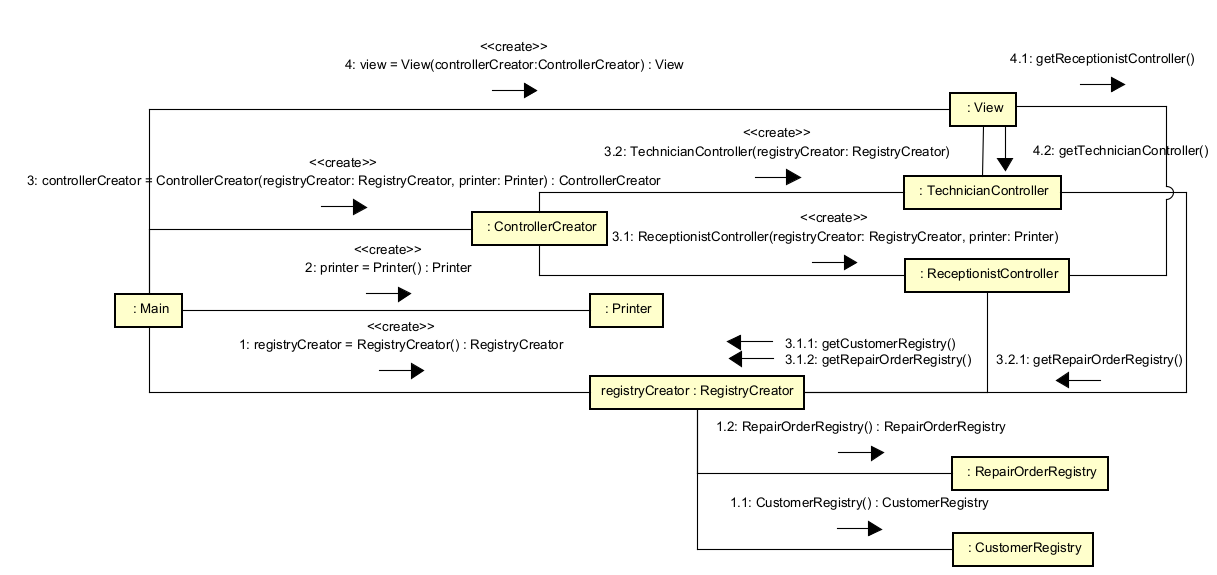
\includegraphics[width=\textwidth]{figures/startup.png}
    \caption{A sample diagram to illustrate caption (this text), numbering and reference in text.}
    \label{fig:diag}
  \end{center}
\end{figure}

\section{Discussion}

\textbf{This chapter evaluates your solution} according to the assessment criteria found in the assessment-criteria documents, which are available under each seminar (sections 4.1-4.4) on the \texttt{Seminar Tasks} page of the course web. To get 2p, it's important that the evaluation is extensive, and \textbf{motivated with concrete examples from your solution}. General statements, that could be applied to any solution, will not contribute to a higher score.

---

\subsection{Evaluation Against Criteria}
The design is evaluated according to Seminar~2 assessment criteria:
\begin{itemize}
  \item \textbf{MVC correctness:} 
        Clear separation between View, Controller, and Model.
  \item \textbf{Encapsulation:}
        DTOs are immutable; domain objects do not leak internal references.
  \item \textbf{Cohesion:}
        Each class has a clear responsibility (e.g.\ 
        \texttt{ProposedRepairTask} handles only task description and cost).
  \item \textbf{Coupling:}
        Controllers depend only on interfaces and DTOs, not internal model structure.
  \item \textbf{Use of exceptions:} 
        Consistent with best practices; user errors vs internal errors separated.
\end{itemize}

\subsection{Limitations and Possible Improvements}
\begin{itemize}
  \item Controller workload could be reduced by introducing service objects.
  \item The DiagnosticReport update process could be made more flexible.
  \item A future data layer could support persistence, indexing, or storage logic.
\end{itemize}

4. Discussion

Goal: Evaluate your design using criteria

4.1 Encapsulation
Are fields private?
Is public interface minimal?
Example from your design
4.2 Cohesion
Do classes have single responsibility?
Example:
RepairOrder handles repair logic only
4.3 Coupling
Are dependencies minimized?
Does controller avoid being “spider-in-the-web”?
4.4 Architecture Evaluation
Does design follow:
MVC?
Layer pattern?
Are responsibilities clearly separated?
4.5 Strengths and Weaknesses

Be specific:

Strengths:
Clear separation of concerns
Scalable design
Weaknesses:
Controller might still be too central
Some coupling to registry layer
4.6 Possible Improvements

Examples:

Move more logic from controller → model
Introduce additional abstractions
Improve handling of repair states

\section*{References}

\textbf{It's mandatory to list here all sources from where you have collected information}, for example course material and YouTube videos. \textbf{Remember that all AI usage must be specified}. There are examples of how AI usage can be specified in Canvas, on the course front page.

You can use any reference style you wish. \textbf{Don't mention other students you have collaborated with}, that shall instead be mentioned in the \textit{Project Members} section at the top of the report.

\end{document}
